
\subsection{Classification}\label{classification}
\subsubsection{Naïve Bayes Classifier}
The Naïve Bayes classifier is a probabilistic classifier based on the Bayes' theorem.
% , having the assumption of independence for each feature. 
Bayes' theorem describes the probability of an event, given some prior knowledge, using the formula:
%is derived from the definition of conditional probability that can be computed using the following formula: 
$P(Class|Sentence)=\frac{P(Sentence|Class)P(Class)}{P(Sentence)}.$
By determining the posteriori probability of \textit{Class}, conditioned by Sentence, we can classify a given instance.

\paragraph{Model Construction}
After preprocessing the text and vectorizing it using TF-IDF, we instantiate a new multinomial Naïve Bayes model using \textit{scikit-learn}\cite{scikit-learn}. We trained the model according to the default settings, with smoothing factor=1.0 and predicted the \textit{class} probability.

\paragraph{Discussion}
This model performs well, obtaining above 80\% accuracy and precision, which means that both TF-IDF and the probabilistic learning process are able to capture the semantics of the text under classification.

\subsubsection{Support Vector Machine}
Support Vector Machine(SVM) is a classification method that although performs very well on linear data, it can also be applied on nonlinear data. The SVM method is designed to search for the optimal linear separating hyperplane using support vectors and margins. The support vectors are training tuples that are correctly labelled, while the margins are defined by the support vectors from different classes. The optimal hyperplane is the one for which the margins are maximal, thus separating the data points under classification.


\paragraph{Model Construction}
% Similarly to the approach of the Naïve Bayes model, we have used the same Python Machine Learning library (\textit{scikit-learn}) to create and train the SVM model. 
We have experimented with a linear kernel with a coefficient of $\frac{1}{\# of features}$ and a regularization parameter of 1.0, also using the \textit{scikit-learn} ML library.

\paragraph{Discussion}
Compared to the previous approach, the linear SVM model seems to perform better, which translates into the representation of the instances under classification being linearly separable in the multi-dimentional space defined by the TF-IDF vectors.

\subsubsection{Neural Network}
We have also applied a neural network technique to classify the reviews. For this model, we have trained embeddings specifically for the text under classification, with the goal of obtaining word embeddings that are suited for the informal style of writing present in this dataset.
The word embeddings obtained using this mechanism have multiple advantages. One of the major advantages is that words that have the same semantic meaning have a similar representation, which is expected to improve the classification performance.

\paragraph{Model Construction}
For this model, we experimented with simple architectures presented in Table \ref{tab:mlp_str} from the Appendices. We have used a sentence length of 74 words, and the dimension of word embeddings 32. The fully connected dense layer has 250 nodes, while the output layer has one neuron (as we are working on binary classification). 

\paragraph{Discussion}
This simple architecture underperforms, according to the results reported in Section \ref{evaluation}, the model not being able to capture the semantic complexity of the text under classification. To improve its performance, there are a number of approaches to be considered as future work such as increasing the embedding dimension, number of training epochs (with mechanisms of early stopping), extending the architecture to multiple layers, and experimenting with different activation functions.

\subsection{Keyword and Key-phrase extraction} \label{keyword}

We started our approach with a baseline, consisting of a bi-LSTM classifier that classifies the input text embedded with GloVe pre-trained embeddings.

We will refer to corpus as the collection of all the training instances for a class: positive or negative.
To gain a better understanding of the semantics of each class's texts, we further applied different statistical and graph-based text mining approaches to extract a dictionary of 300 key-words and key-phrases for each of the two corpora (positive and negative). As an alternative, we have also report the results obtained by applying these techniques on each review and then ranking the keyphrases based on their assigned scores.
While for the implementation of the algorithms described in the following sections we have used python libraries (\textit{yake}, \textit{rake-nltk}, and \textit{pytextrank}), our contributions focus on the design of the evaluation model described in Section \ref{generator}. 
\subsubsection{Statistical methods}
\paragraph{TF-IDF}
One of the most common numerical statistic is TF-IDF (described in section \ref{tfidf}). We use this approach to compute the score of each term in a review (document), ranking the scores of the resulting keywords and preserving the top 300 candidates.
\paragraph{RAKE} (Rapid Automatic Keyword Extraction) \cite{rake} is a statistical domain-independent approach that uses both the frequencies and the co-occurrences of the words. The score of each word is computed as the ratio between its frequency and the degree of the word in the matrix of co-occurrences (the sum of the number of co-occurrences the word has with any other content word in the text).      
\paragraph{YAKE} \cite{yake} is a language-independent single document keyword extraction algorithm that uses the following features: Casing, Word Positional, Word Frequency, Word Relatedness to Context, and Word DifSentence to heuristically compute a score for each keyword candidate. For n-grams, the score is divided by the term frequency of the keyword. The resulting similar candidates are filtered out based on the Levenshtein \cite{Levenshtein} distance and ranked based on the score, outputting 1,2 and 3-grams.
\subsubsection{Graph-based methods}
\paragraph{TextRank}
TextRank is an unsupervised graph-based method proposed in 2004 \cite{TextRank}. This method builds a graph where each node represents a lexical unit (one word), as a keyword candidate. The edges between the nodes are added when the words are situated in a window of maximum $N$ words in the original document, where $N$ is a hyperparameter. The scores computed based on the number of edges between the nodes are then sorted in decreasing order and the top $k$ keywords are extracted. The hyperparameter $k$ is set to a third of the number of the total words in the input text. In a post-processing phase, the selected keywords that are adjacent in the original document are grouped to form multi-word expressions.

\subsection{Sentiment Analysis Keyword Generator}\label{generator}
After building the dictionary of possible key-terms candidates, we design a MLP generator that outputs a probability distribution over the dictionaries. The one-hot encoding of it is further used to select the key-phrase that the baseline bi-LSTM classifier uses to improve its confidence on the classification task.
For a better understanding, we provide an architectural diagram in Figure \ref{fig:gen}.


\begin{figure}[!h]
\centering
  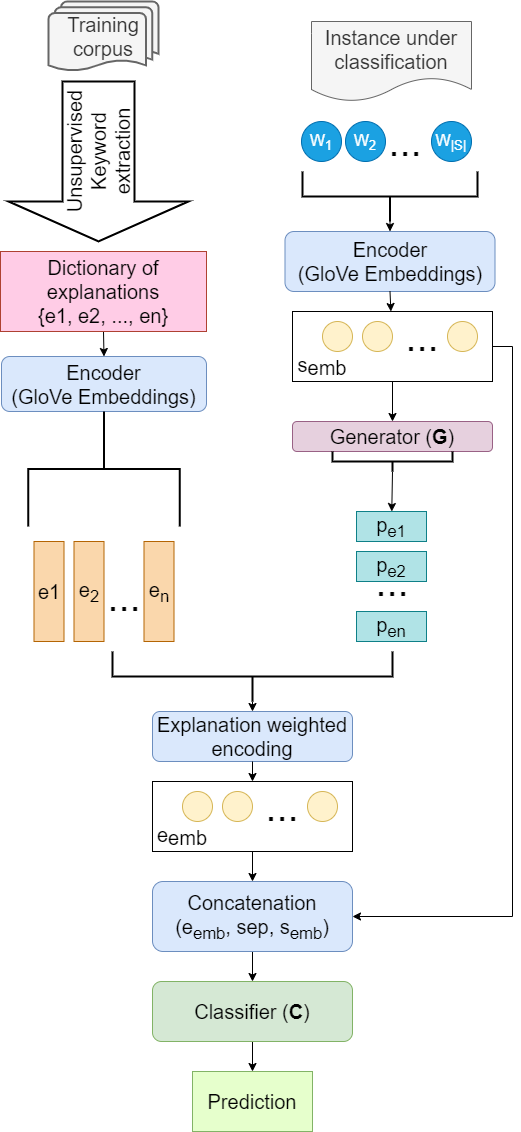
\includegraphics[width=5cm]{Images/gen.png}
  \caption{Generator architecture}\label{fig:gen}
\end{figure}